\documentclass{beamer}
\usepackage{graphicx}
\usepackage{color}

\usetheme{Berlin}
\usecolortheme{beaver}
\title[A constant current applied to the HH model produces a train of action potentials.]{Step current responce of the HH Model}

\author[E.Ioannidis \& J.Hobin] {\
   \texorpdfstring{\
        \begin{columns}
            \column{.45\linewidth}
            \centering
            Eleftherios Ioannidis\\
            \href{mailto:elefthei@mit.edu}{elefthei@mit.edu}
            \column{.45\linewidth}
            \centering
            James Hobin\\
            \href{mailto:hobinjk@mit.edu}{hobinjk@mit.edu}
        \end{columns}
   }
   {Eleftherios Ioannidis \& James Hobin}
}


\institute{MIT EECS}
\date{\today}

% ============================================
% DOCUMENT BEGINING HERE
% ============================================

\begin{document}

% Title slide (1)
\begin{frame}
  \titlepage{}
\end{frame}

\begin{frame}{HH Model Step Current Responce}
  \begin{figure}
    \centering
    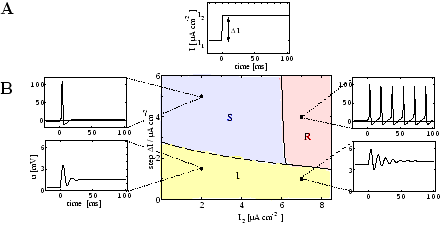
\includegraphics[width = 0.8\textwidth]{./pictures/gerstner.png}
    \caption{Step Current Stimulation Phase diagram}
  \end{figure}
\end{frame}

\begin{frame}{Applications: Refractory Period}
  \begin{figure}
    \centering
    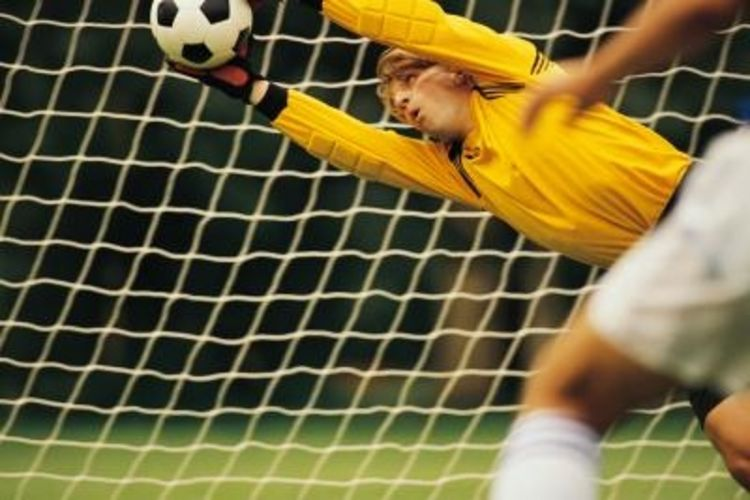
\includegraphics[width = 0.4\textwidth]{./pictures/reflexes.jpg}
    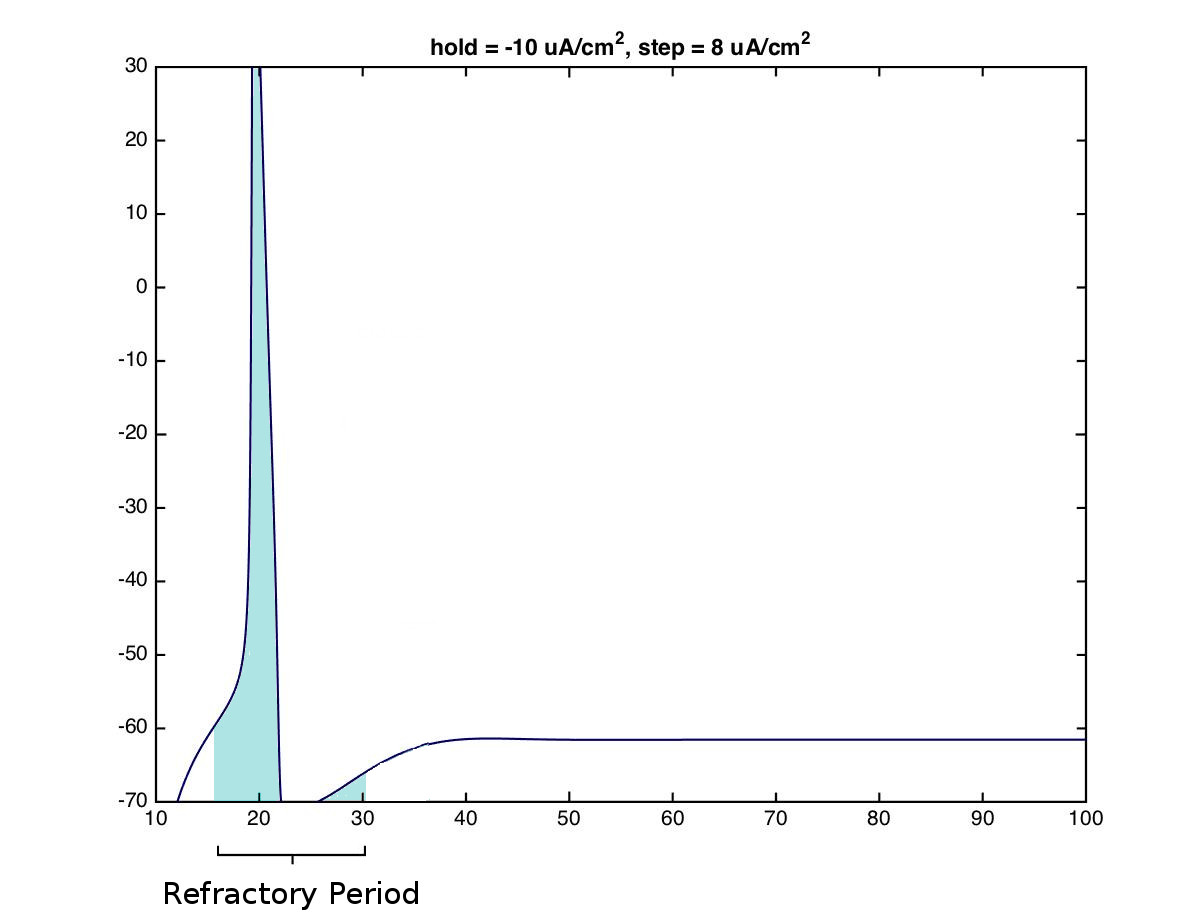
\includegraphics[width = 0.6\textwidth]{./pictures/refractory.jpg}
    \caption{Reducing the Refractory Period can lead to faster reflexes.}
  \end{figure}
\end{frame}



\begin{frame}
  \begin{figure}
    \centering
    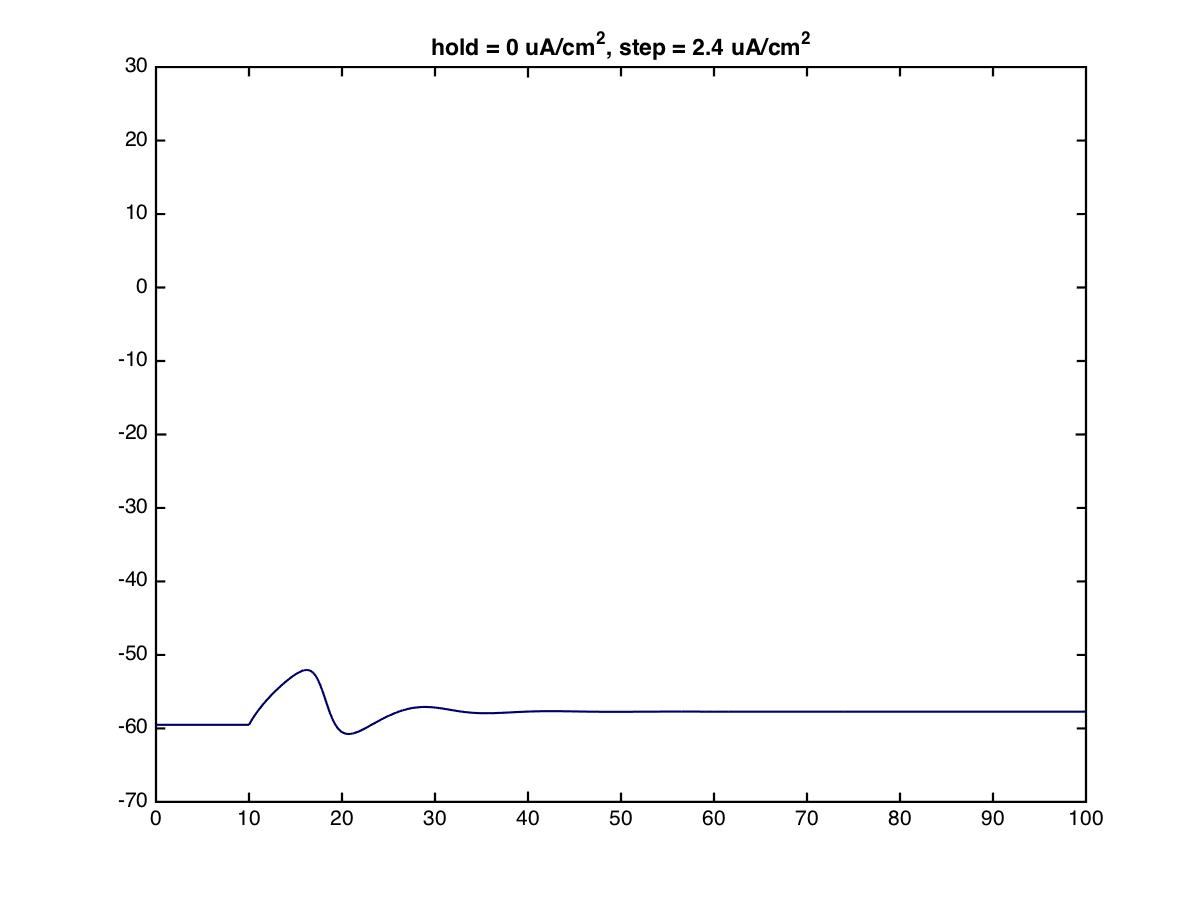
\includegraphics[width = 0.33\textwidth]{./images/current_0_2p4.jpg}
    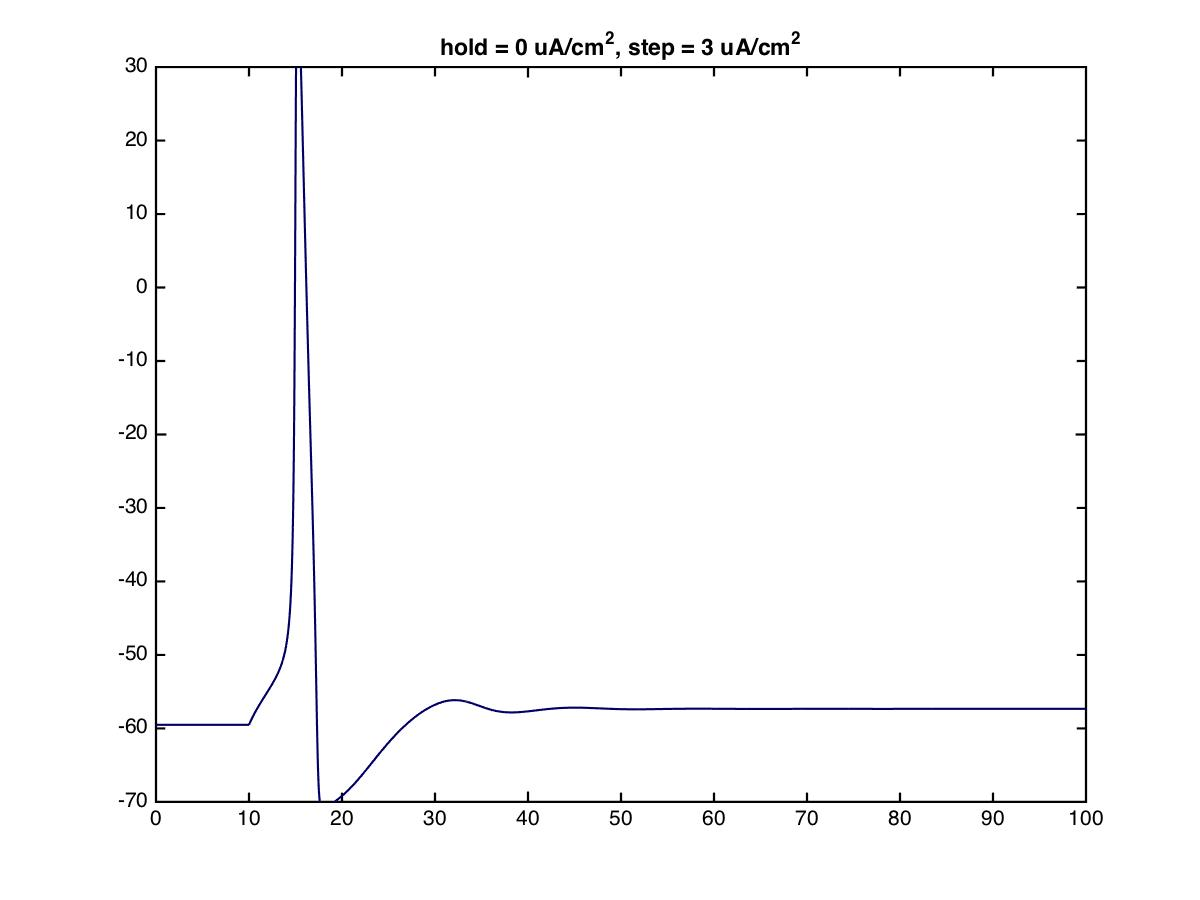
\includegraphics[width = 0.33\textwidth]{./images/current_0_3.jpg}
    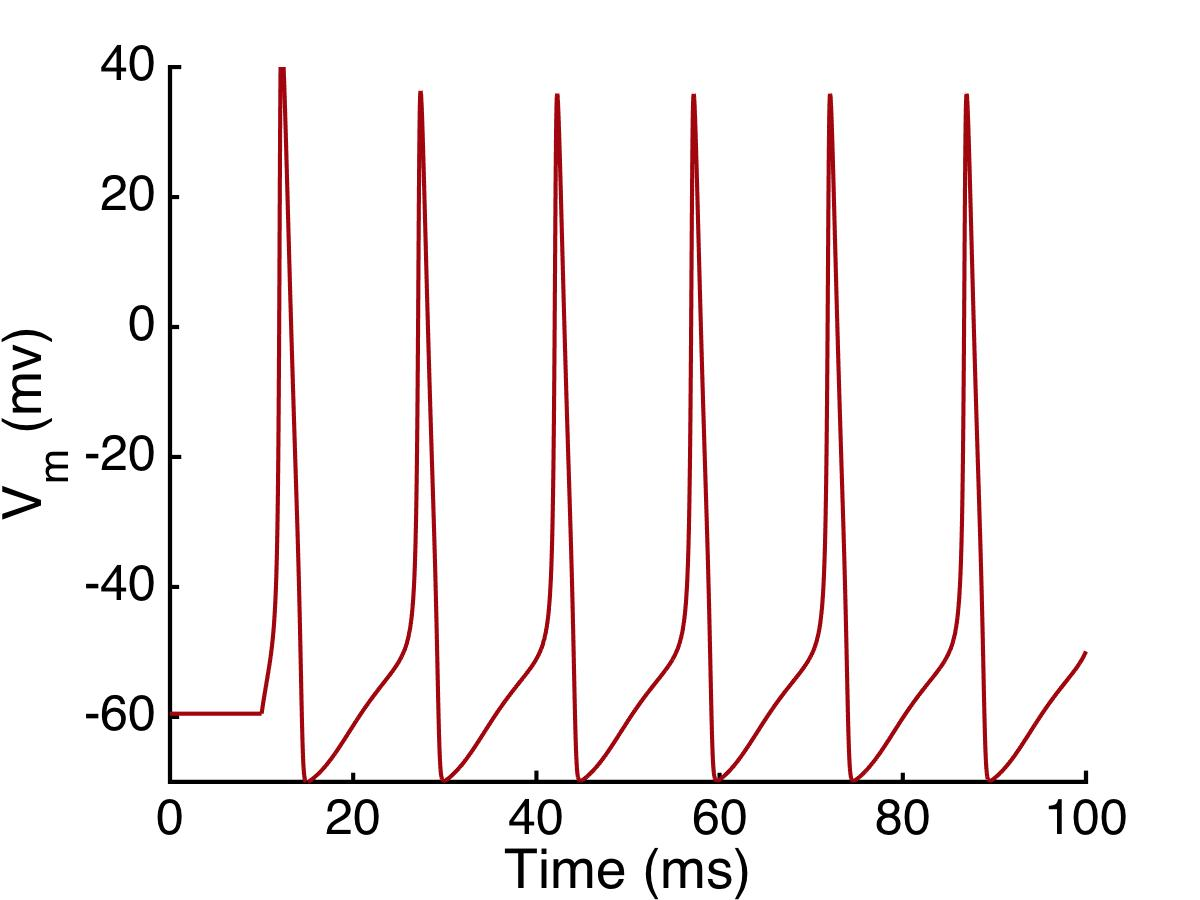
\includegraphics[width = 0.33\textwidth]{./images/current_0_10.jpg}
    \caption{Response in the \emph{Ringing}, \emph{Single AP} and \emph{AP Train} regions}
  \end{figure}
\end{frame}

% slide 0
\begin{frame}
  \begin{figure}
    \centering
    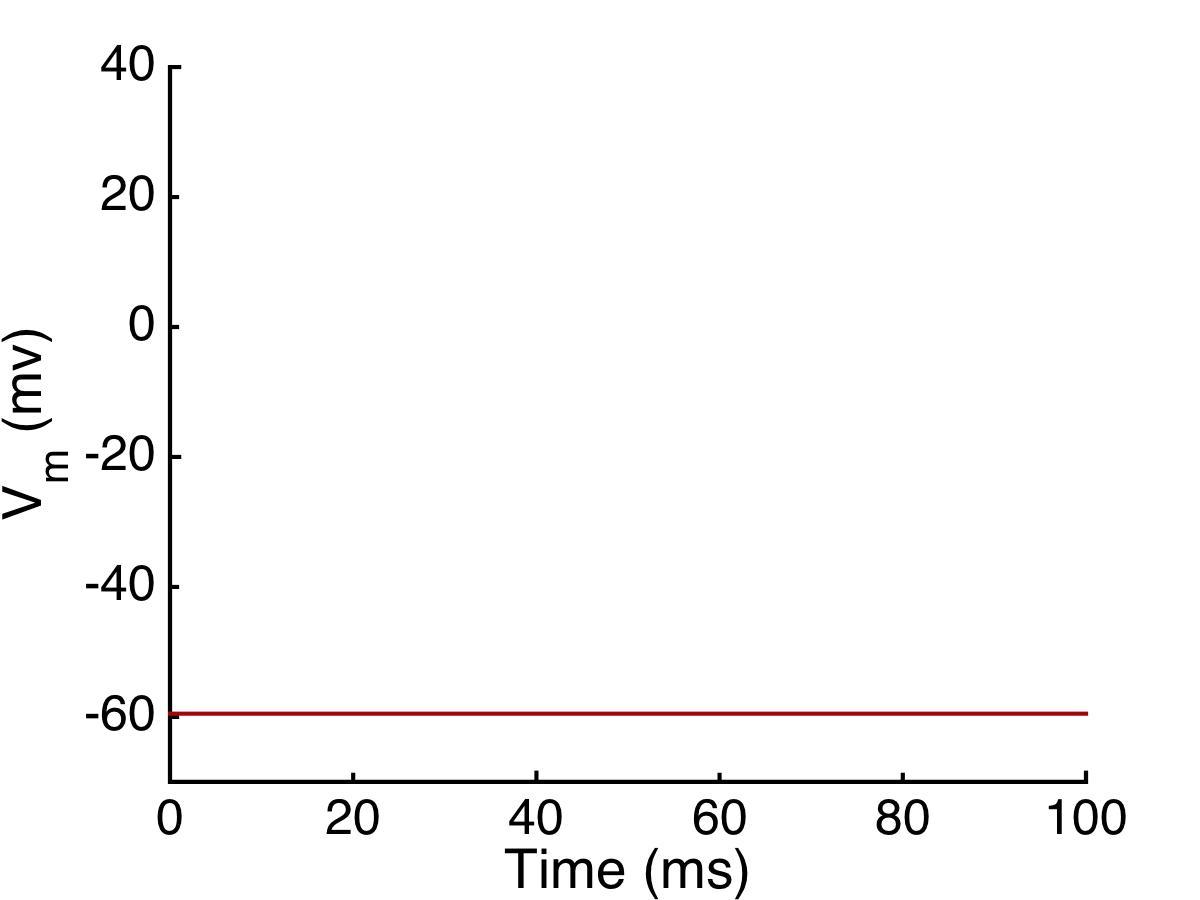
\includegraphics[width = 0.8\textwidth]{./images/current_0_0.jpg}
    \caption{HH Models step current response starting at 0 $\mu A/cm^2$}
  \end{figure}
\end{frame}


% slide 5
\begin{frame}
  \begin{figure}
    \centering
    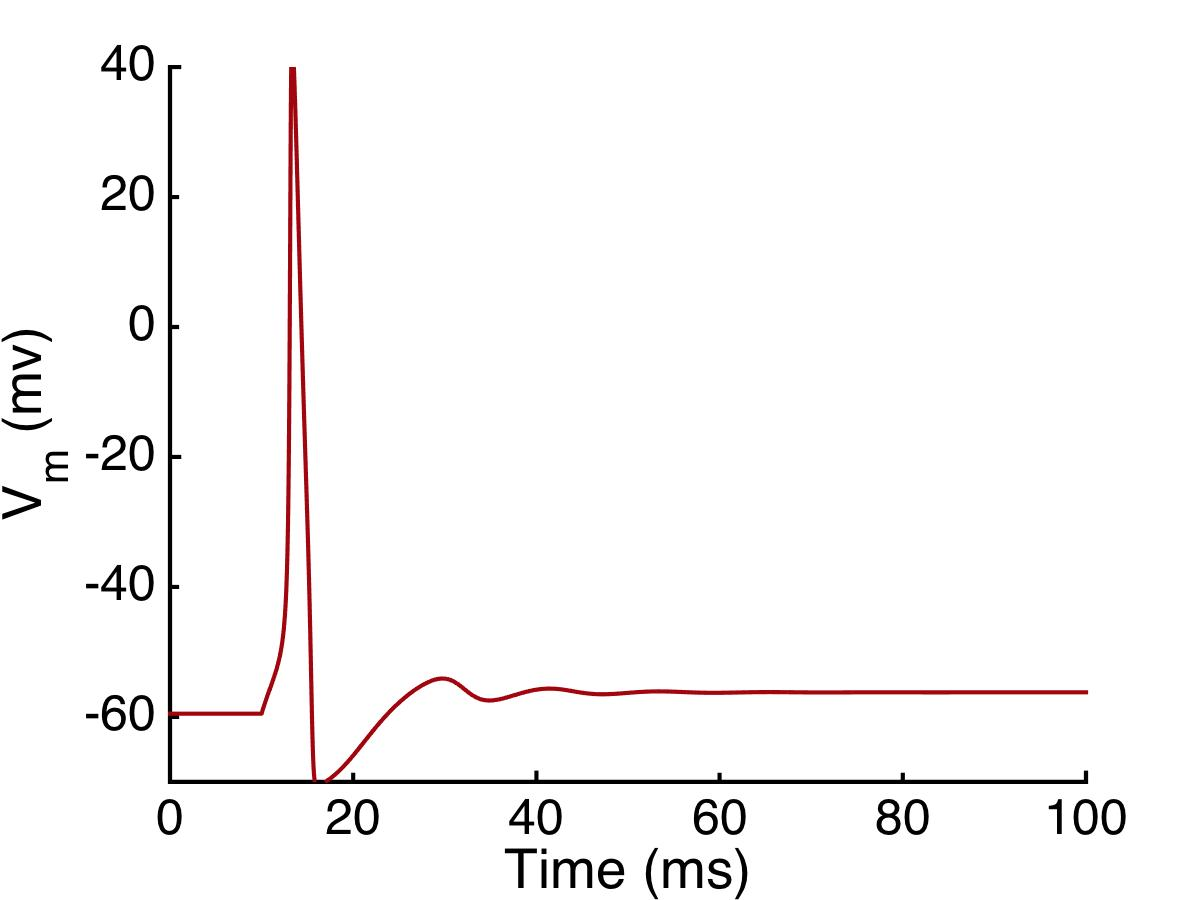
\includegraphics[width = 0.8\textwidth]{./images/current_0_5.jpg}
    \caption{HH Models step current response starting at 0 $\mu A/cm^2$}
  \end{figure}
\end{frame}


% slide 10
\begin{frame}
  \begin{figure}
    \centering
    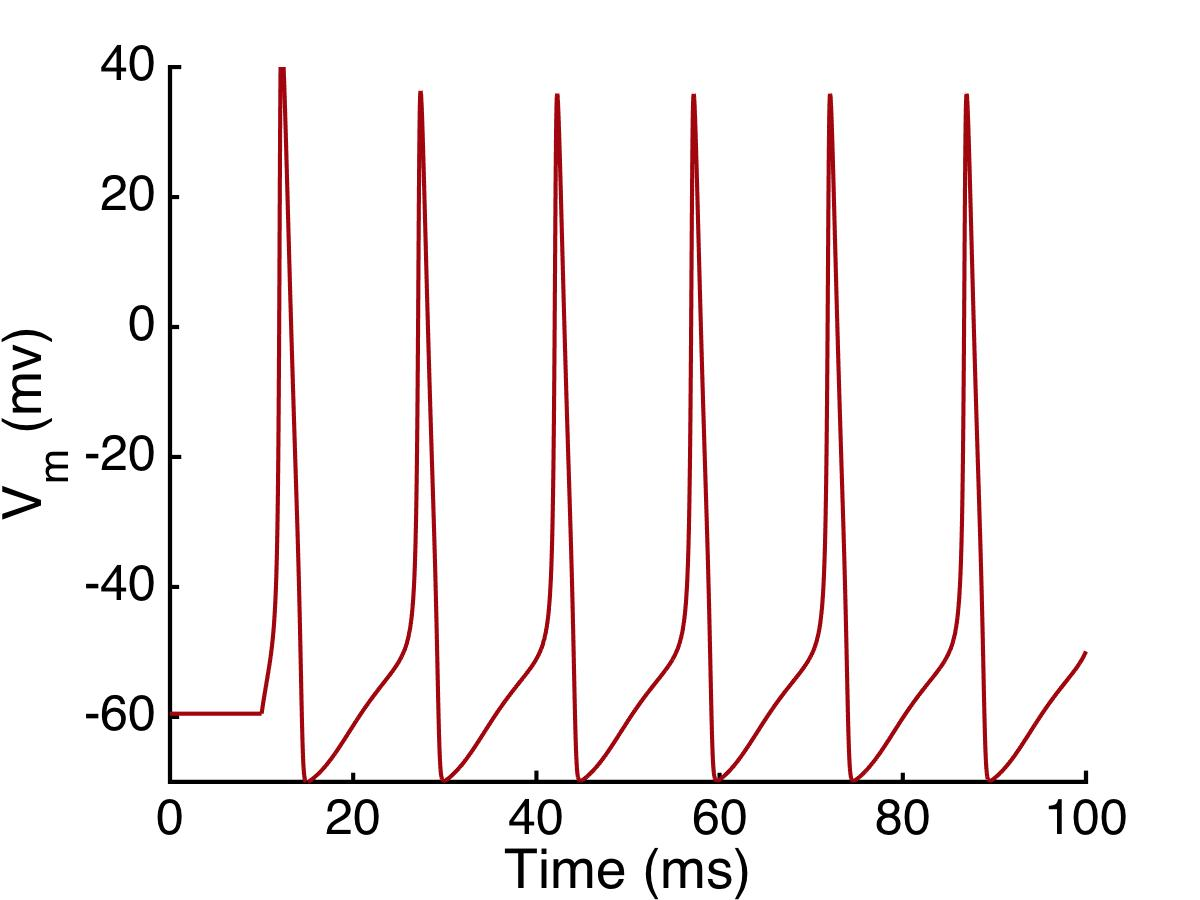
\includegraphics[width = 0.8\textwidth]{./images/current_0_10.jpg}
    \caption{HH Models step current response starting at 0 $\mu A/cm^2$}
  \end{figure}
\end{frame}


% slide 15
\begin{frame}
  \begin{figure}
    \centering
    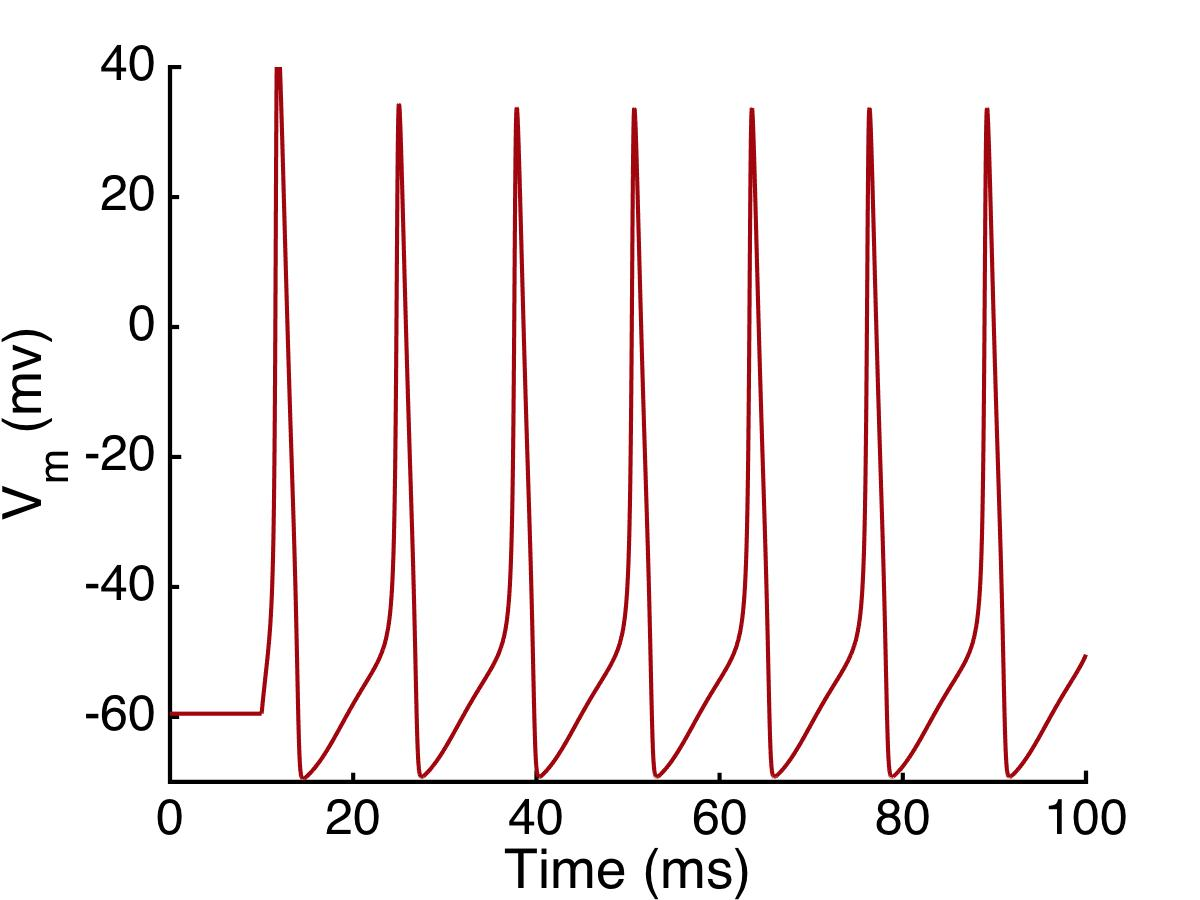
\includegraphics[width = 0.8\textwidth]{./images/current_0_15.jpg}
    \caption{HH Models step current response starting at 0 $\mu A/cm^2$}
  \end{figure}
\end{frame}


% slide 20
\begin{frame}
  \begin{figure}
    \centering
    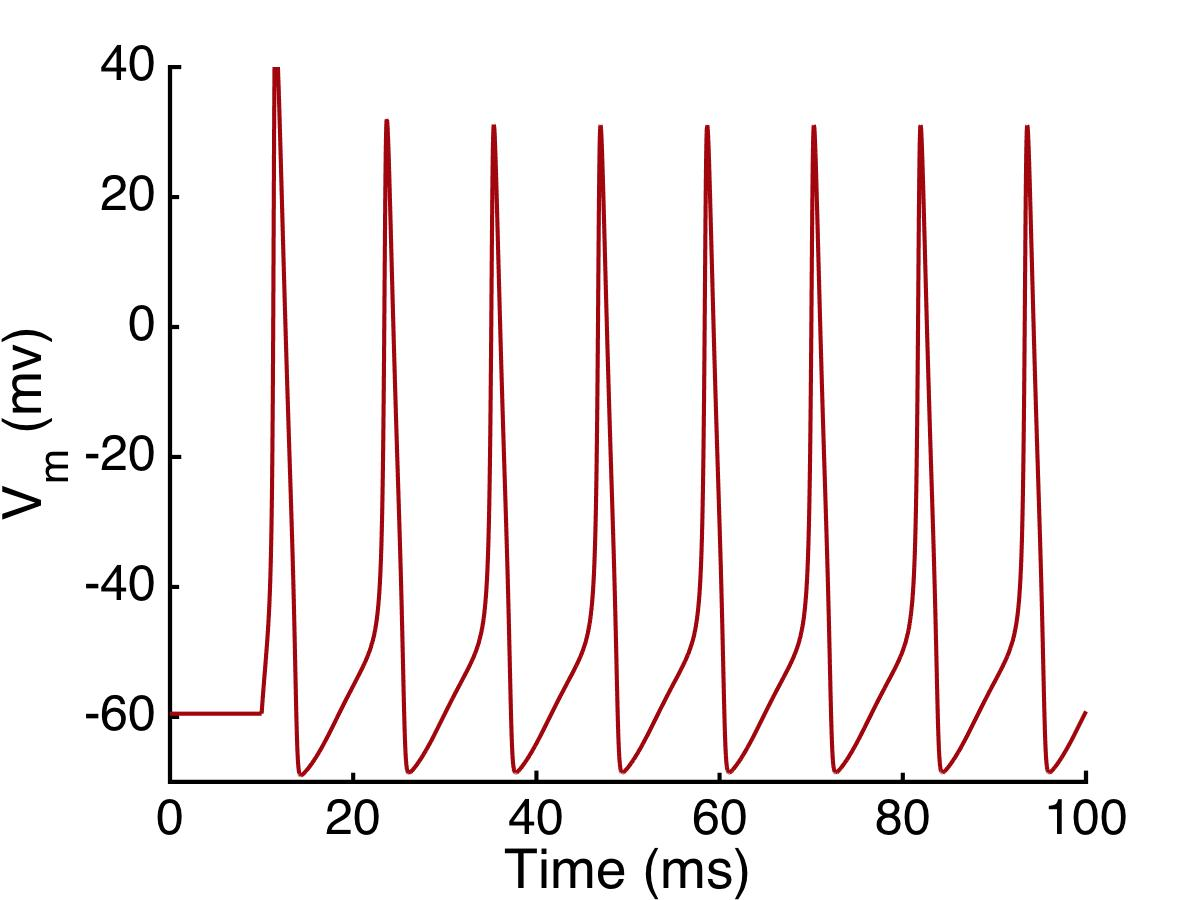
\includegraphics[width = 0.8\textwidth]{./images/current_0_20.jpg}
    \caption{HH Models step current response starting at 0 $\mu A/cm^2$}
  \end{figure}
\end{frame}


% slide 25
\begin{frame}
  \begin{figure}
    \centering
    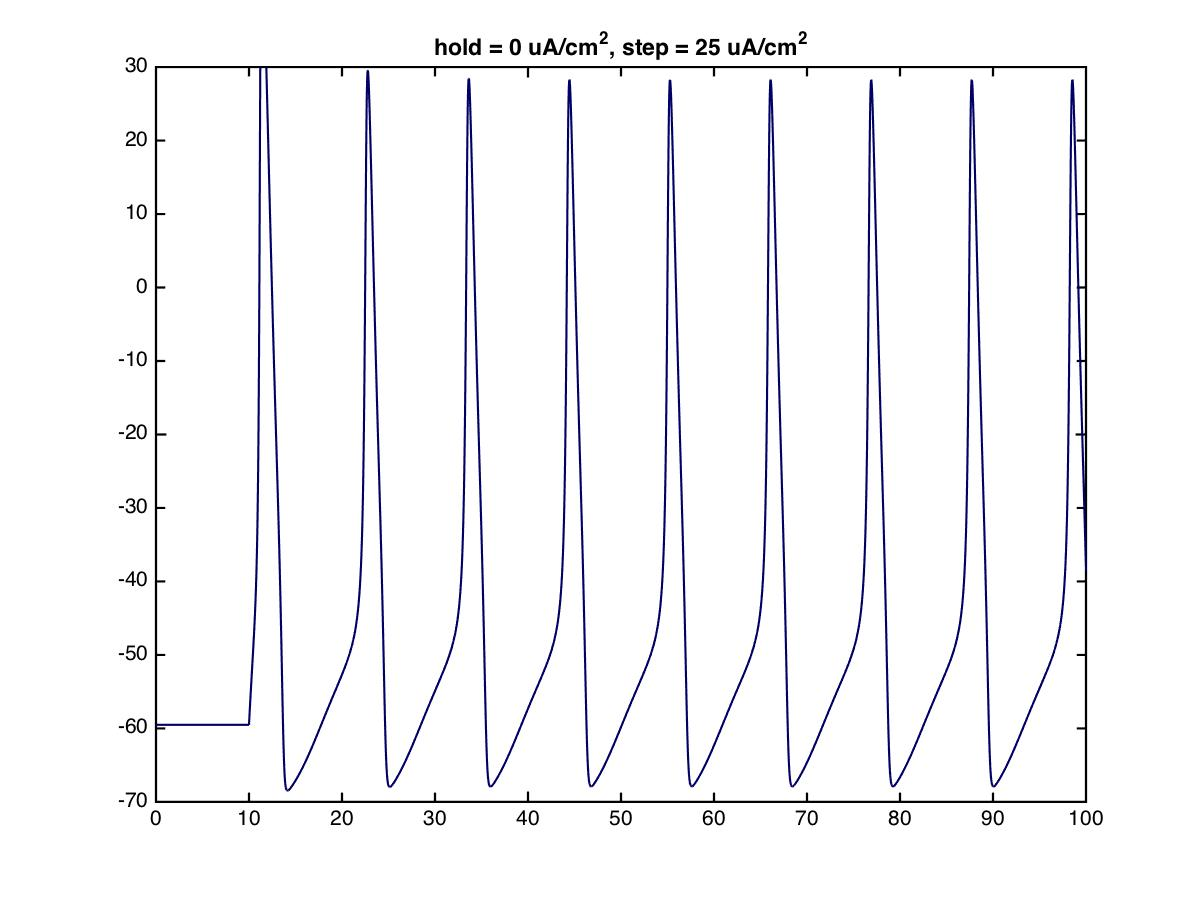
\includegraphics[width = 0.8\textwidth]{./images/current_0_25.jpg}
    \caption{HH Models step current response starting at 0 $\mu A/cm^2$}
  \end{figure}
\end{frame}


% slide 30
\begin{frame}
  \begin{figure}
    \centering
    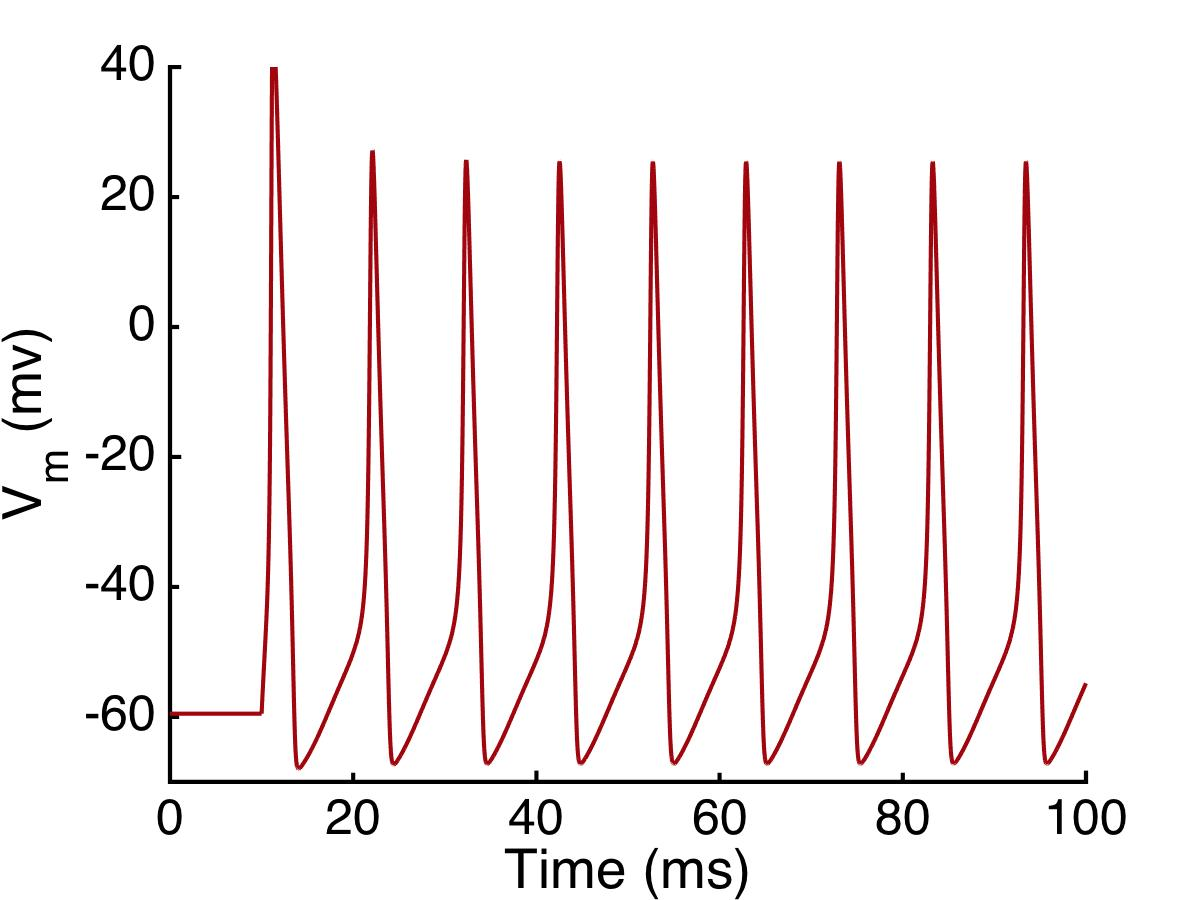
\includegraphics[width = 0.8\textwidth]{./images/current_0_30.jpg}
    \caption{HH Models step current response starting at 0 $\mu A/cm^2$}
  \end{figure}
\end{frame}


% slide 35
\begin{frame}
  \begin{figure}
    \centering
    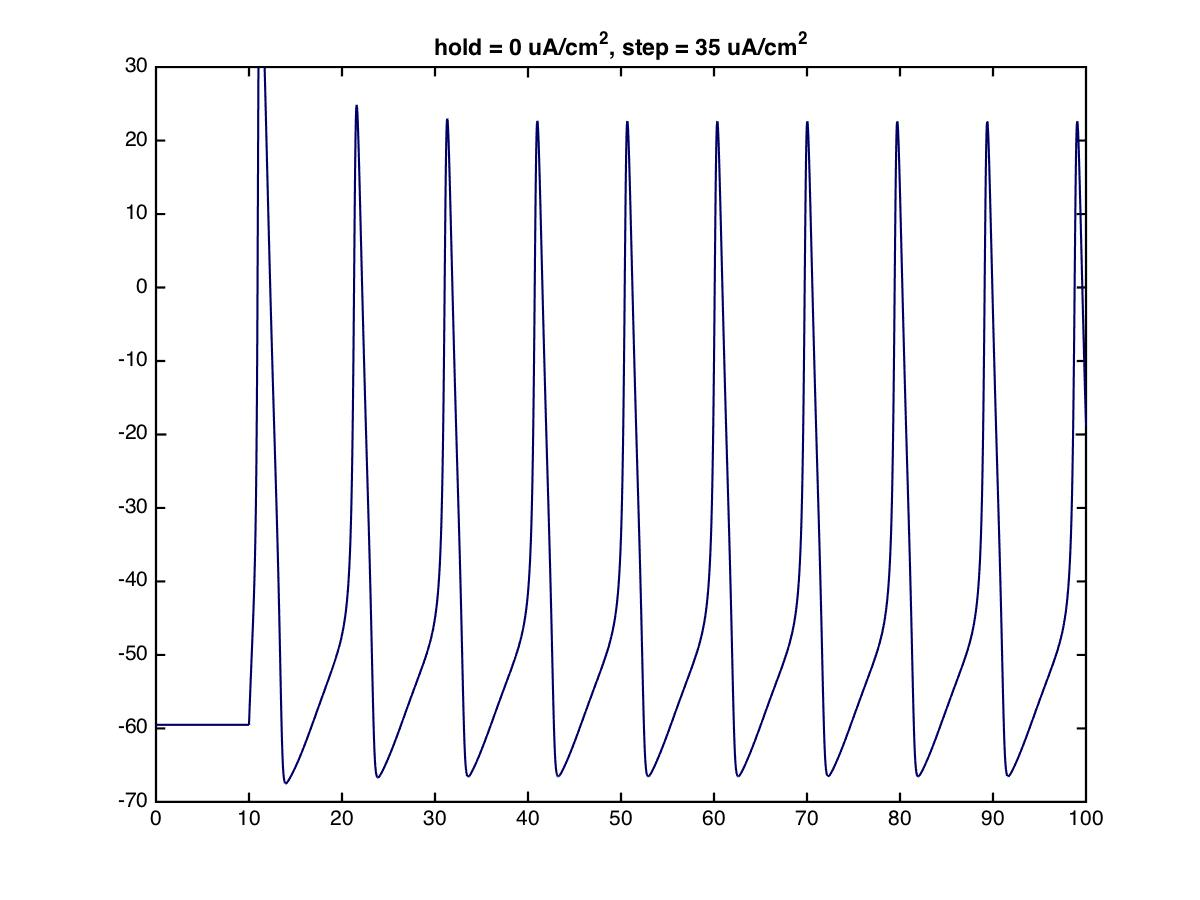
\includegraphics[width = 0.8\textwidth]{./images/current_0_35.jpg}
    \caption{HH Models step current response starting at 0 $\mu A/cm^2$}
  \end{figure}
\end{frame}

% slide 40
\begin{frame}
  \begin{figure}
    \centering
    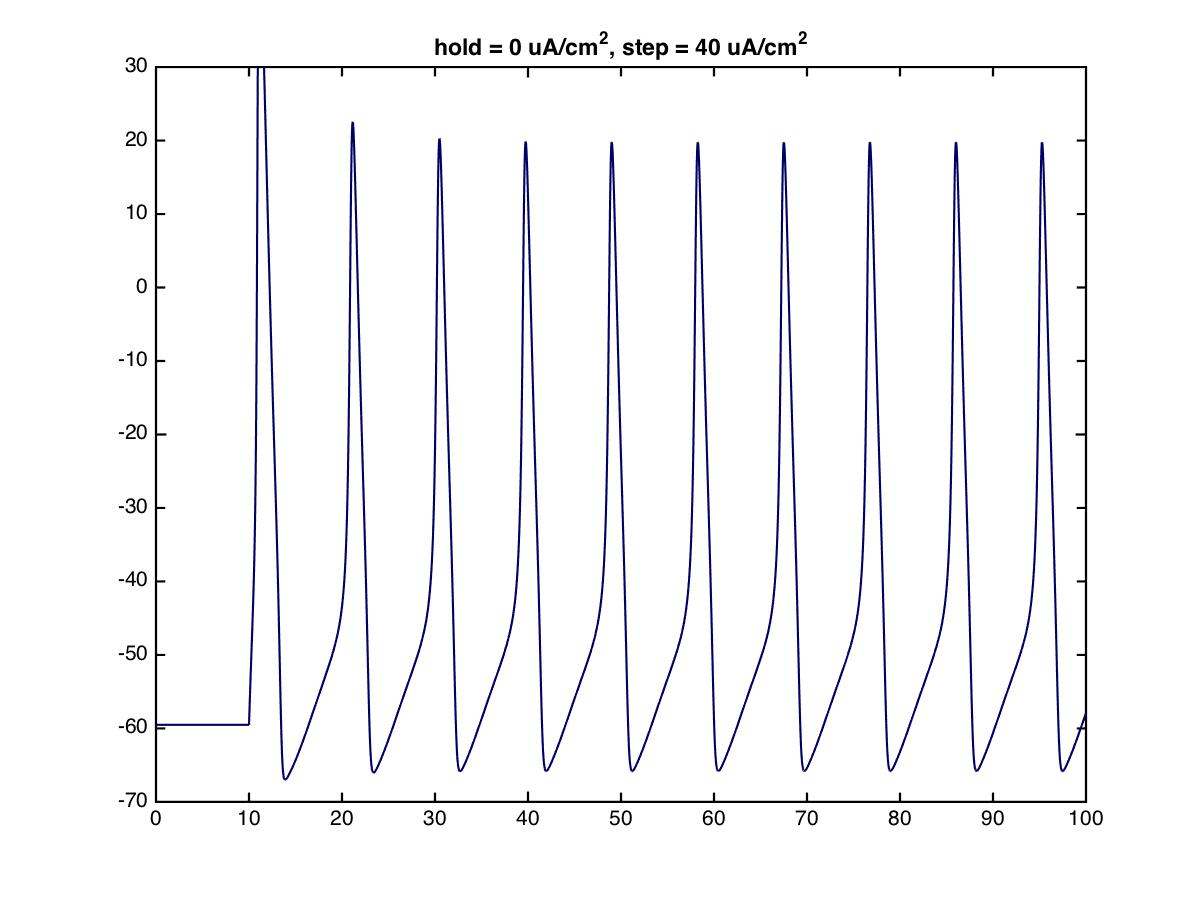
\includegraphics[width = 0.8\textwidth]{./images/current_0_40.jpg}
    \caption{HH Models step current response starting at 0 $\mu A/cm^2$}
  \end{figure}
\end{frame}


% slide 45
\begin{frame}
  \begin{figure}
    \centering
    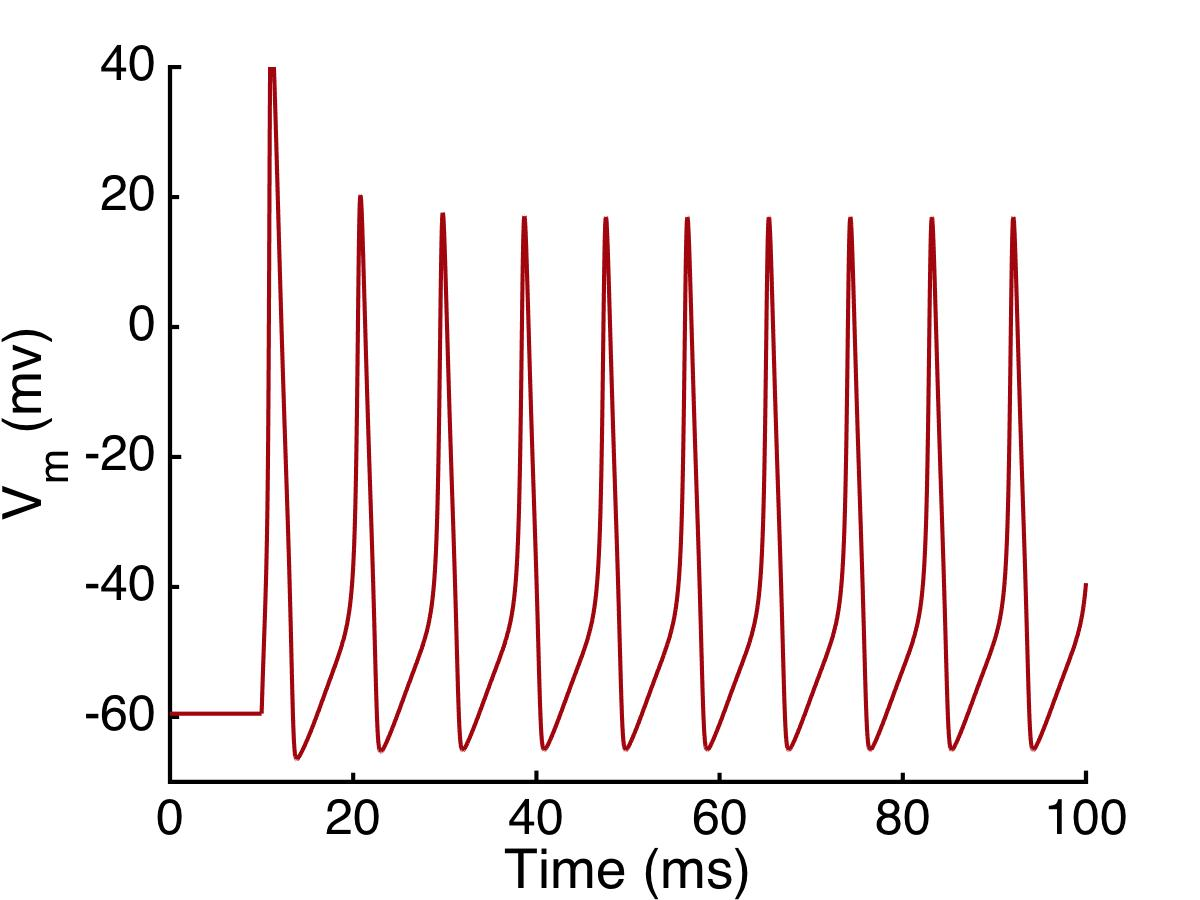
\includegraphics[width = 0.8\textwidth]{./images/current_0_45.jpg}
    \caption{HH Models step current response starting at 0 $\mu A/cm^2$}
  \end{figure}
\end{frame}


% slide 50
\begin{frame}
  \begin{figure}
    \centering
    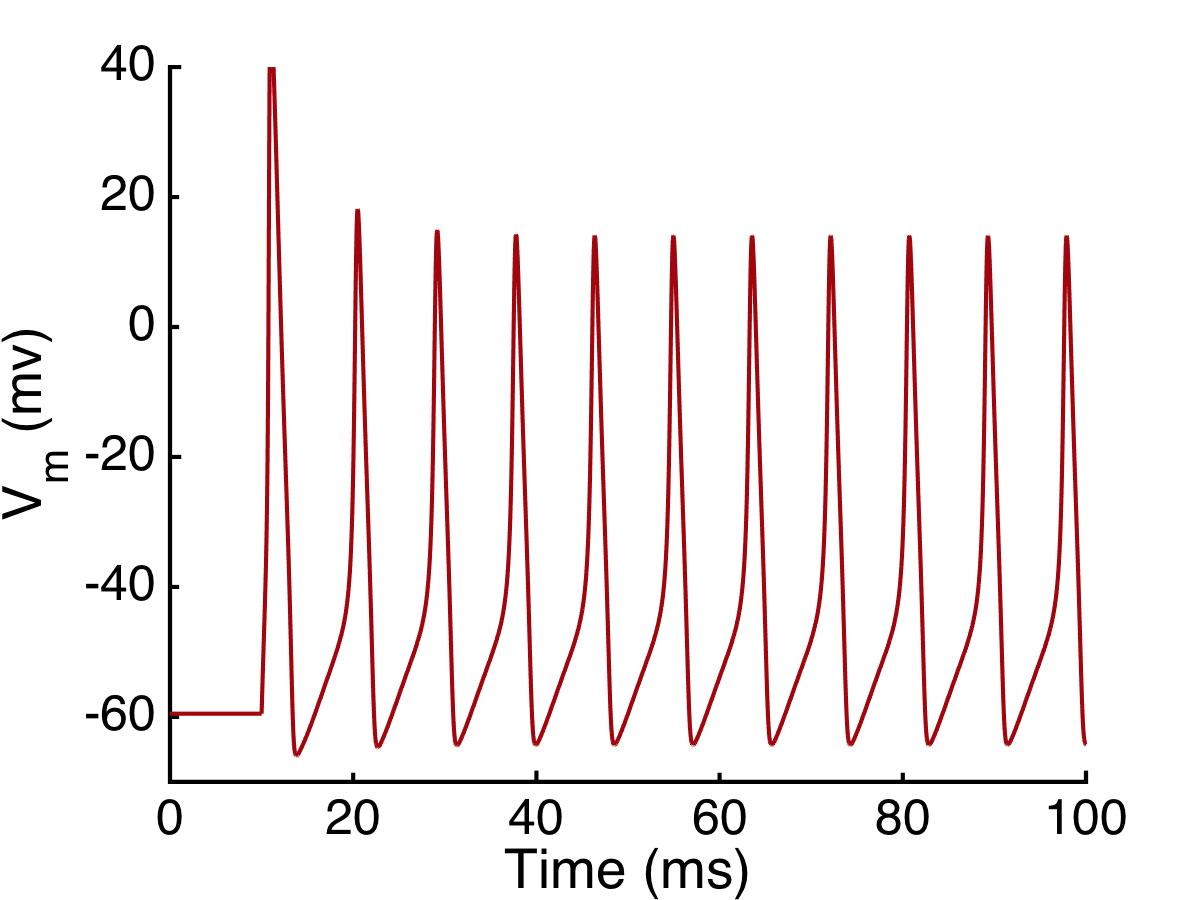
\includegraphics[width = 0.8\textwidth]{./images/current_0_50.jpg}
    \caption{HH Models step current response starting at 0 $\mu A/cm^2$}
  \end{figure}
\end{frame}


% slide 55
\begin{frame}
  \begin{figure}
    \centering
    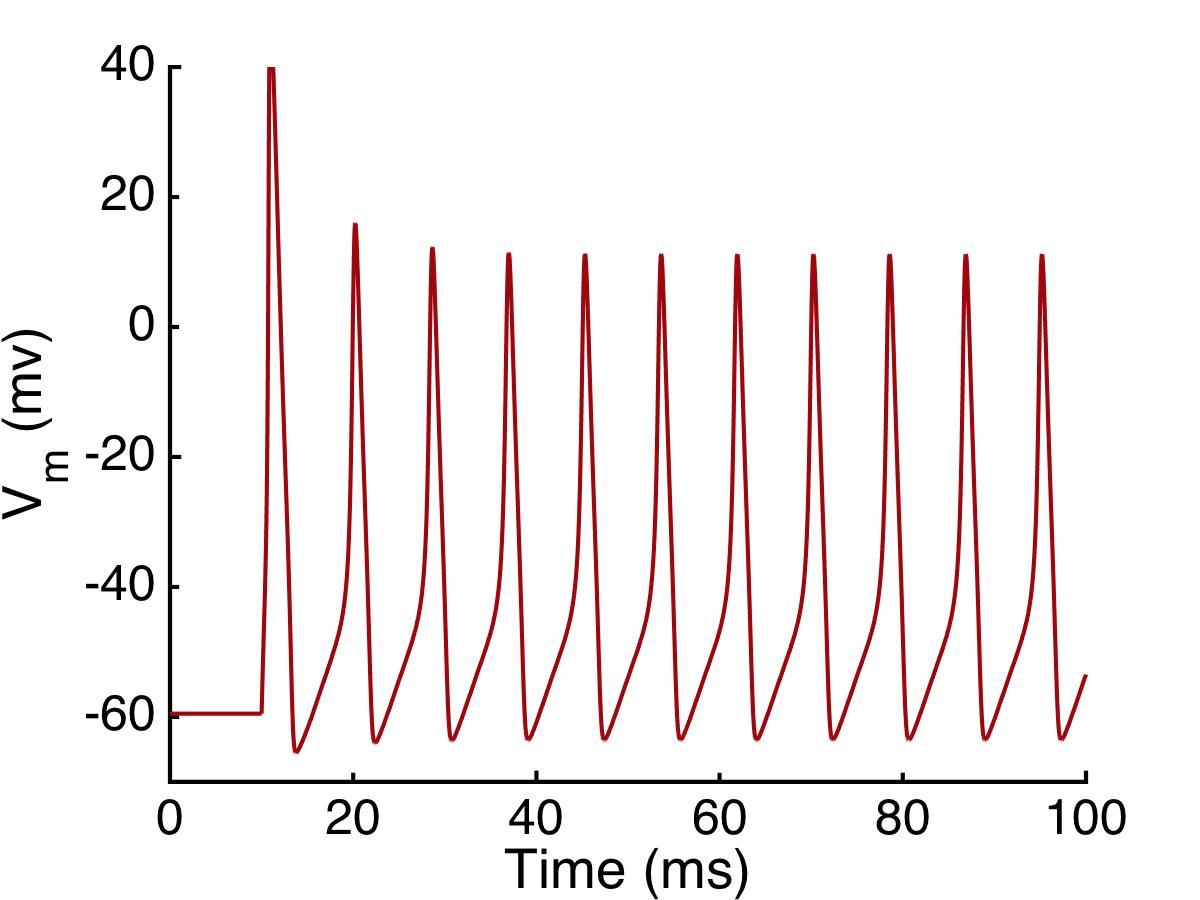
\includegraphics[width = 0.8\textwidth]{./images/current_0_55.jpg}
    \caption{HH Models step current response starting at 0 $\mu A/cm^2$}
  \end{figure}
\end{frame}


% slide 60
\begin{frame}
  \begin{figure}
    \centering
    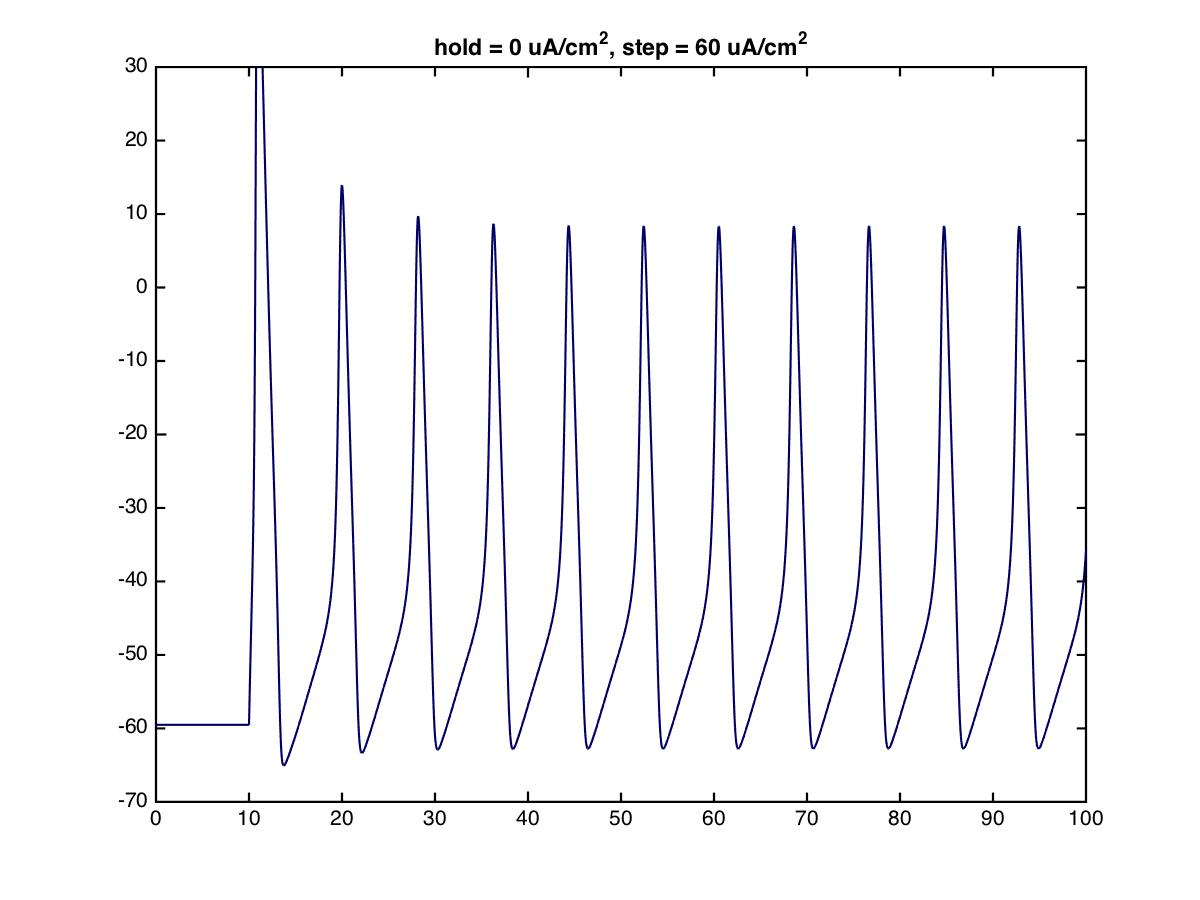
\includegraphics[width = 0.8\textwidth]{./images/current_0_60.jpg}
    \caption{HH Models step current response starting at 0 $\mu A/cm^2$}
  \end{figure}
\end{frame}


% slide 65
\begin{frame}
  \begin{figure}
    \centering
    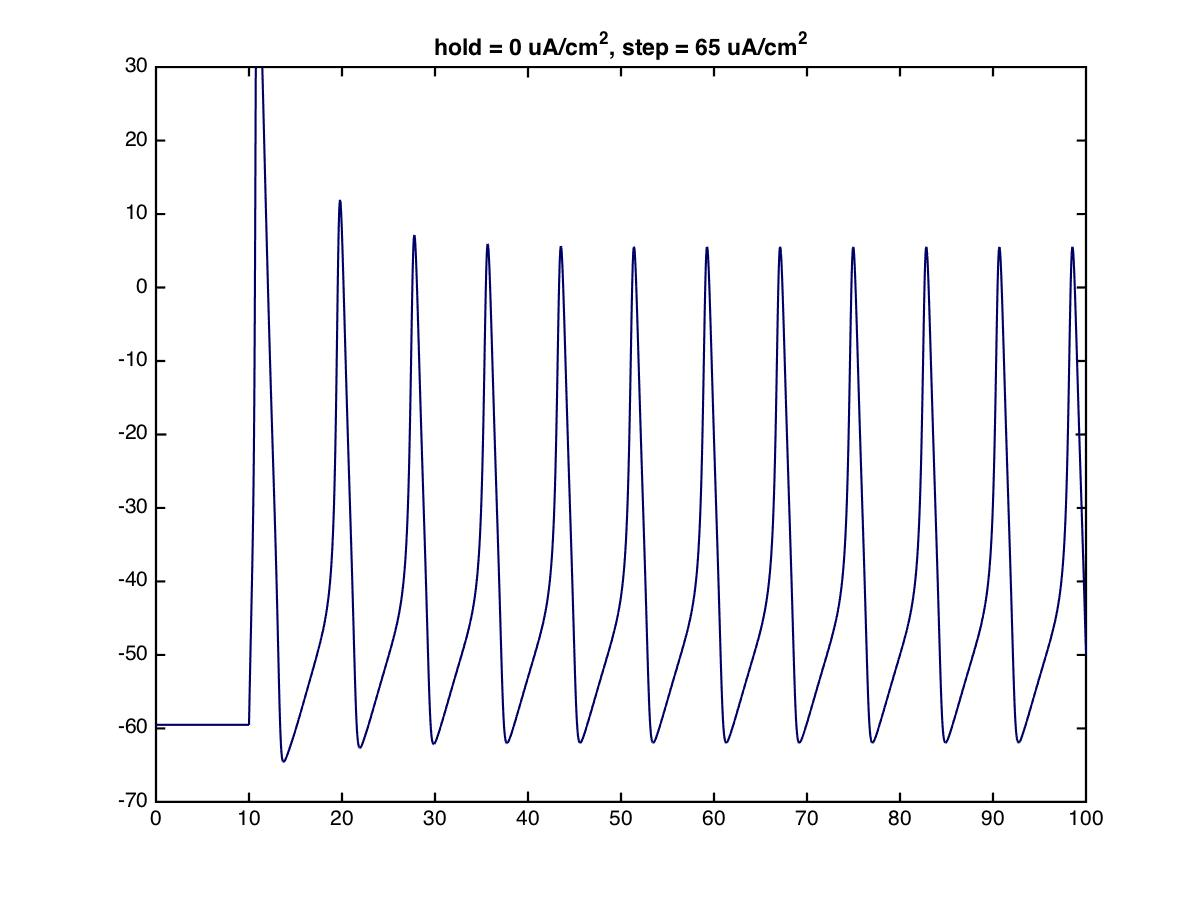
\includegraphics[width = 0.8\textwidth]{./images/current_0_65.jpg}
    \caption{HH Models step current response starting at 0 $\mu A/cm^2$}
  \end{figure}
\end{frame}


% slide 70
\begin{frame}
  \begin{figure}
    \centering
    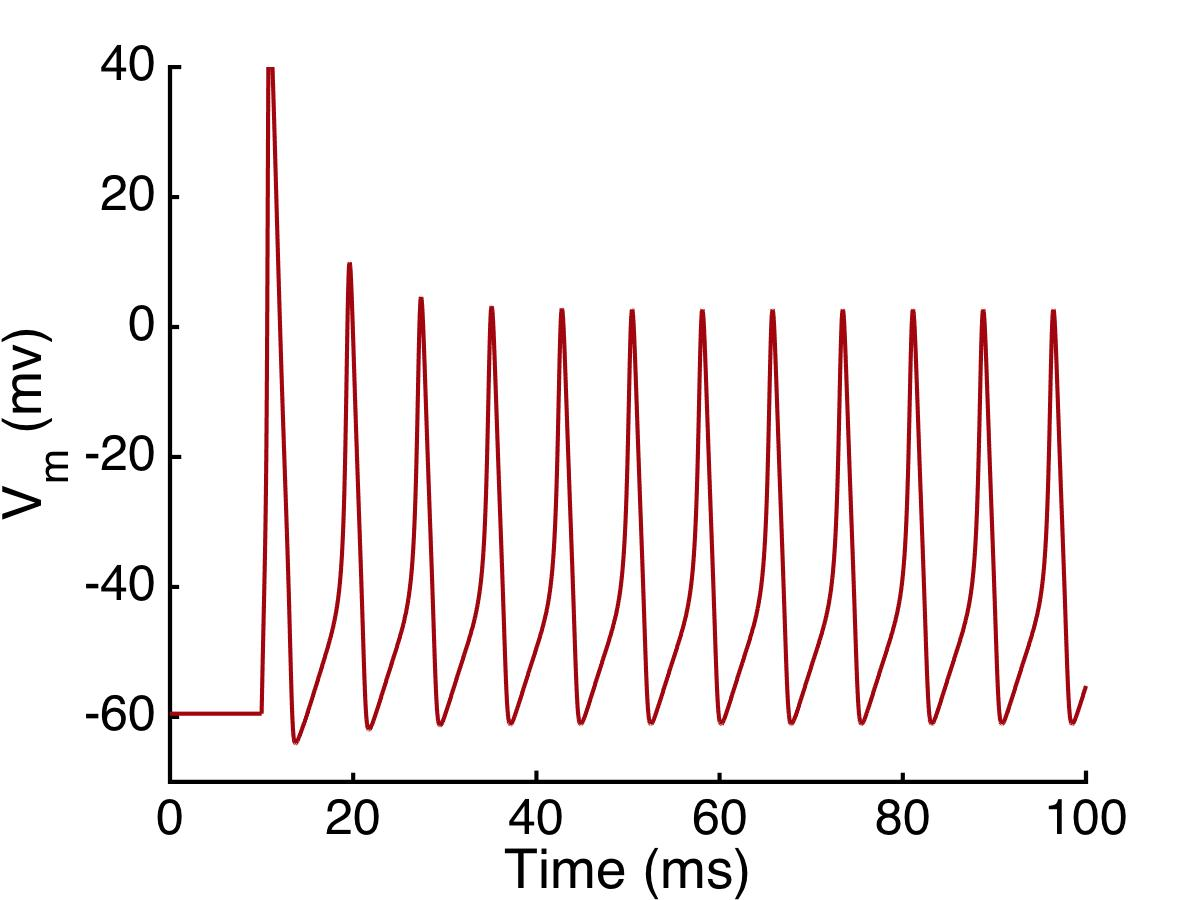
\includegraphics[width = 0.8\textwidth]{./images/current_0_70.jpg}
    \caption{HH Models step current response starting at 0 $\mu A/cm^2$}
  \end{figure}
\end{frame}


% slide 75
\begin{frame}
  \begin{figure}
    \centering
    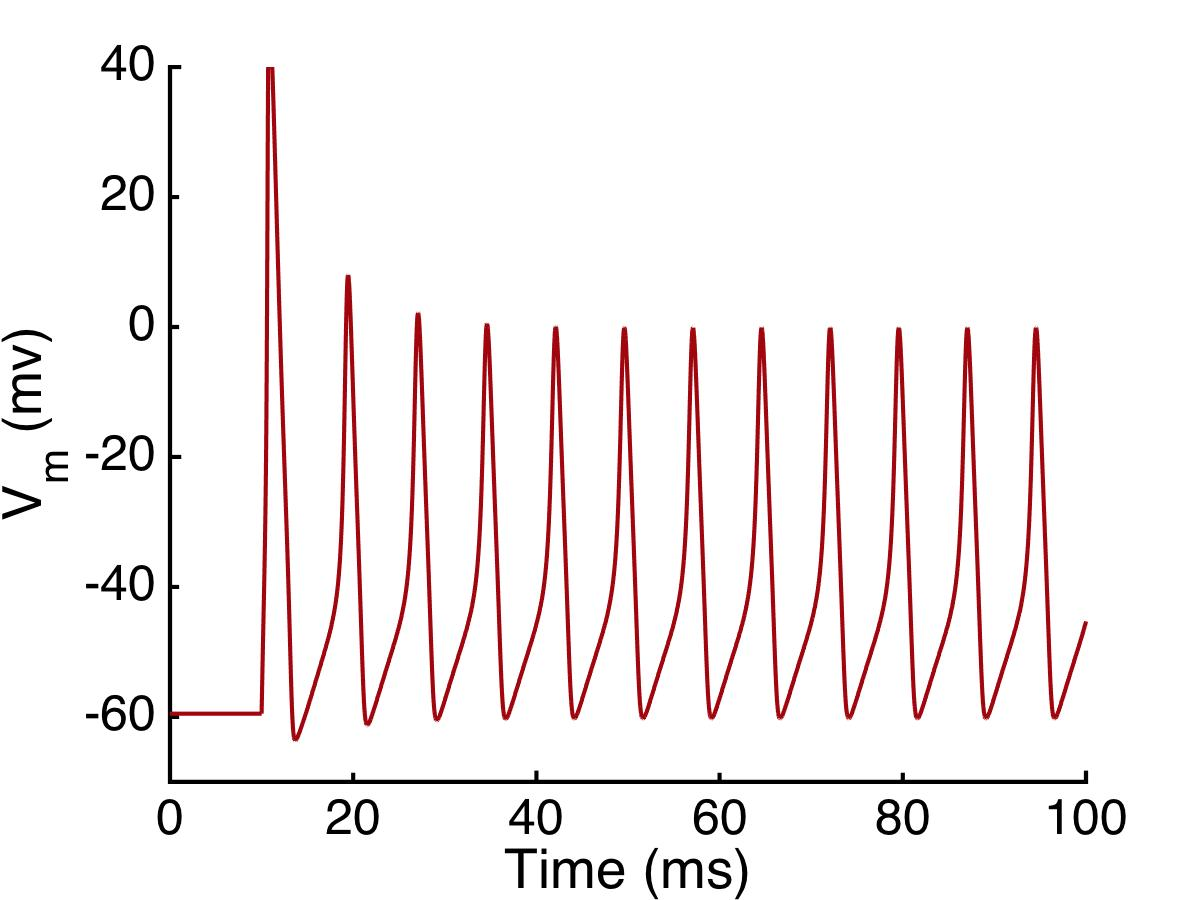
\includegraphics[width = 0.8\textwidth]{./images/current_0_75.jpg}
    \caption{HH Models step current response starting at 0 $\mu A/cm^2$}
  \end{figure}
\end{frame}


% slide 80
\begin{frame}
  \begin{figure}
    \centering
    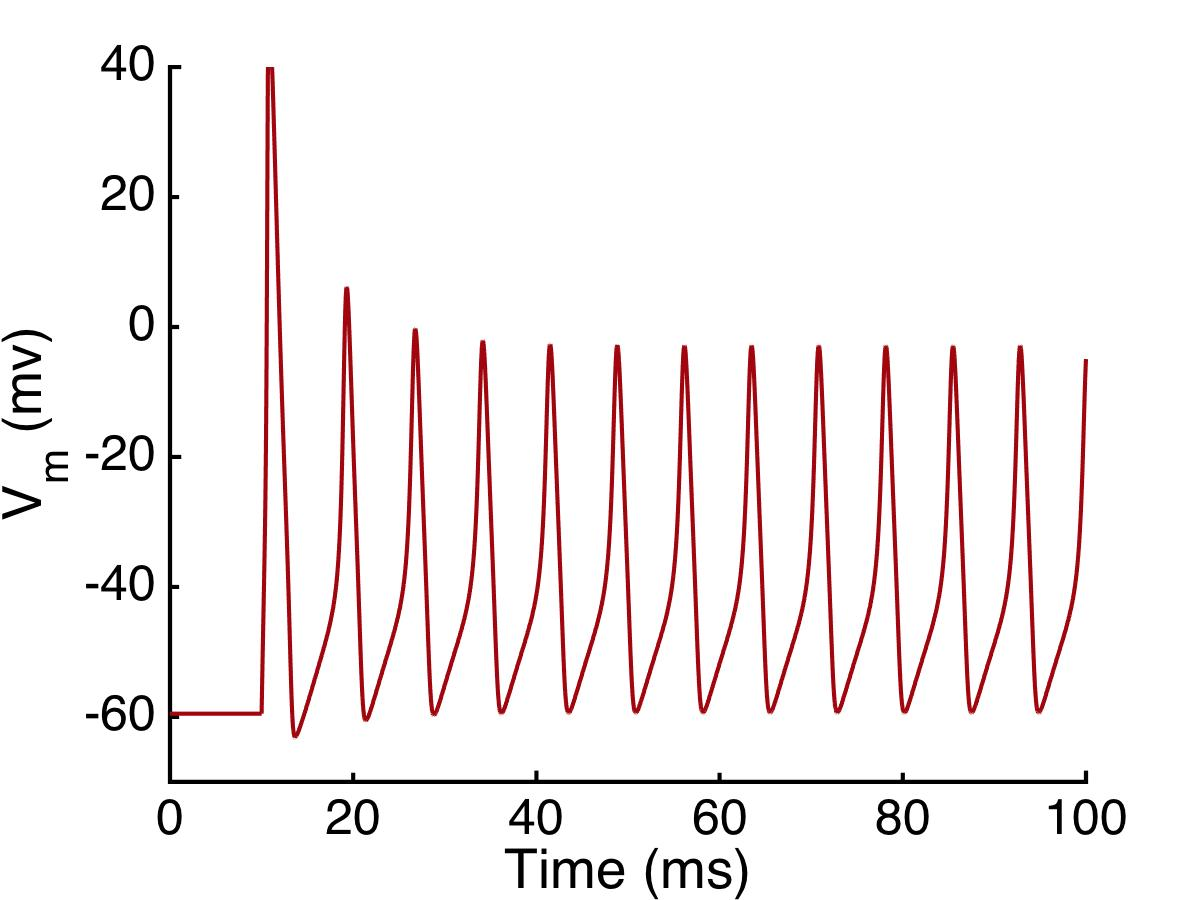
\includegraphics[width = 0.8\textwidth]{./images/current_0_80.jpg}
    \caption{HH Models step current response starting at 0 $\mu A/cm^2$}
  \end{figure}
\end{frame}

\begin{frame}{DFT insufficient}
  \begin{figure}
    \centering
    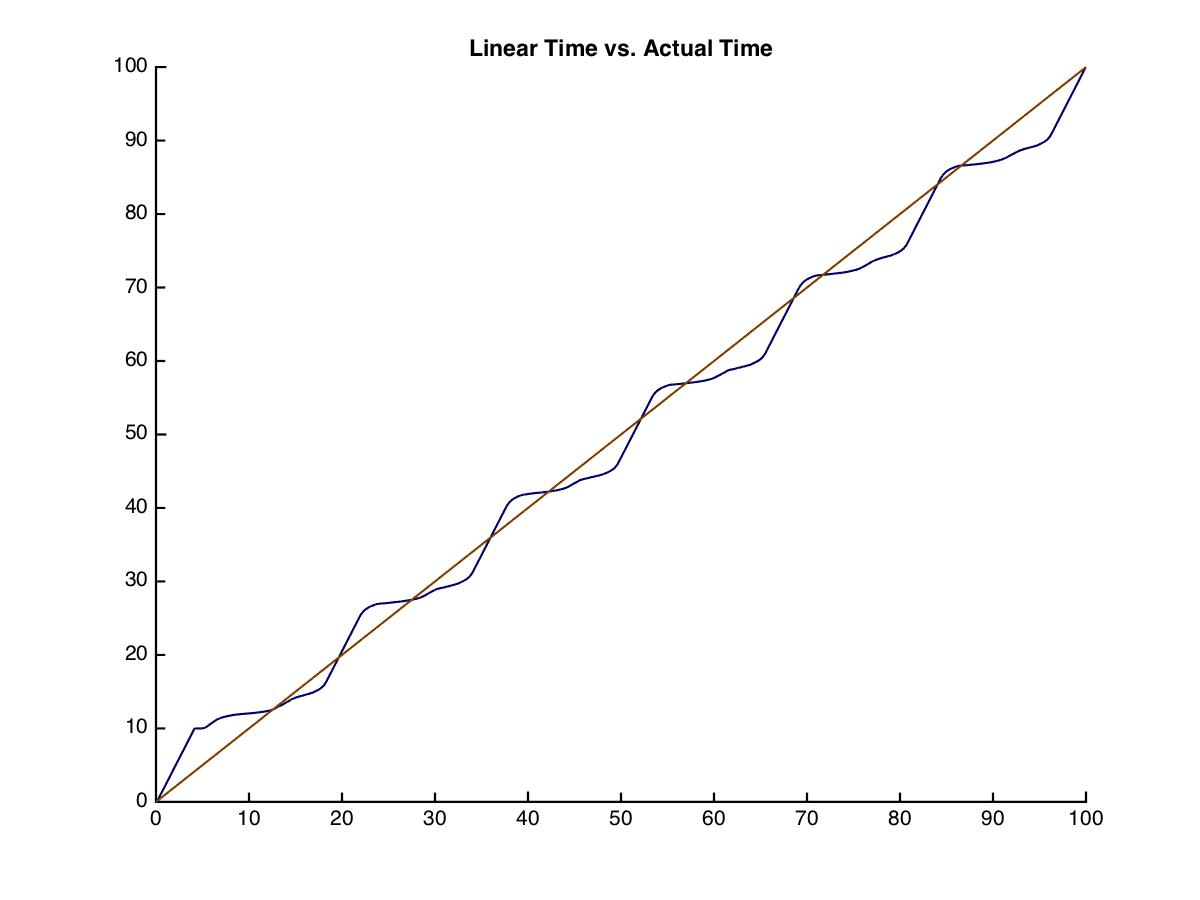
\includegraphics[width = 0.8\textwidth]{./images/lintimevsactualtime.jpg}
    \caption{Discrete Fourier Transform insufficient due to variable time intervals.}
  \end{figure}
\end{frame}

\begin{frame}{Least-squares spectral analysis}
  \begin{figure}
    \centering
    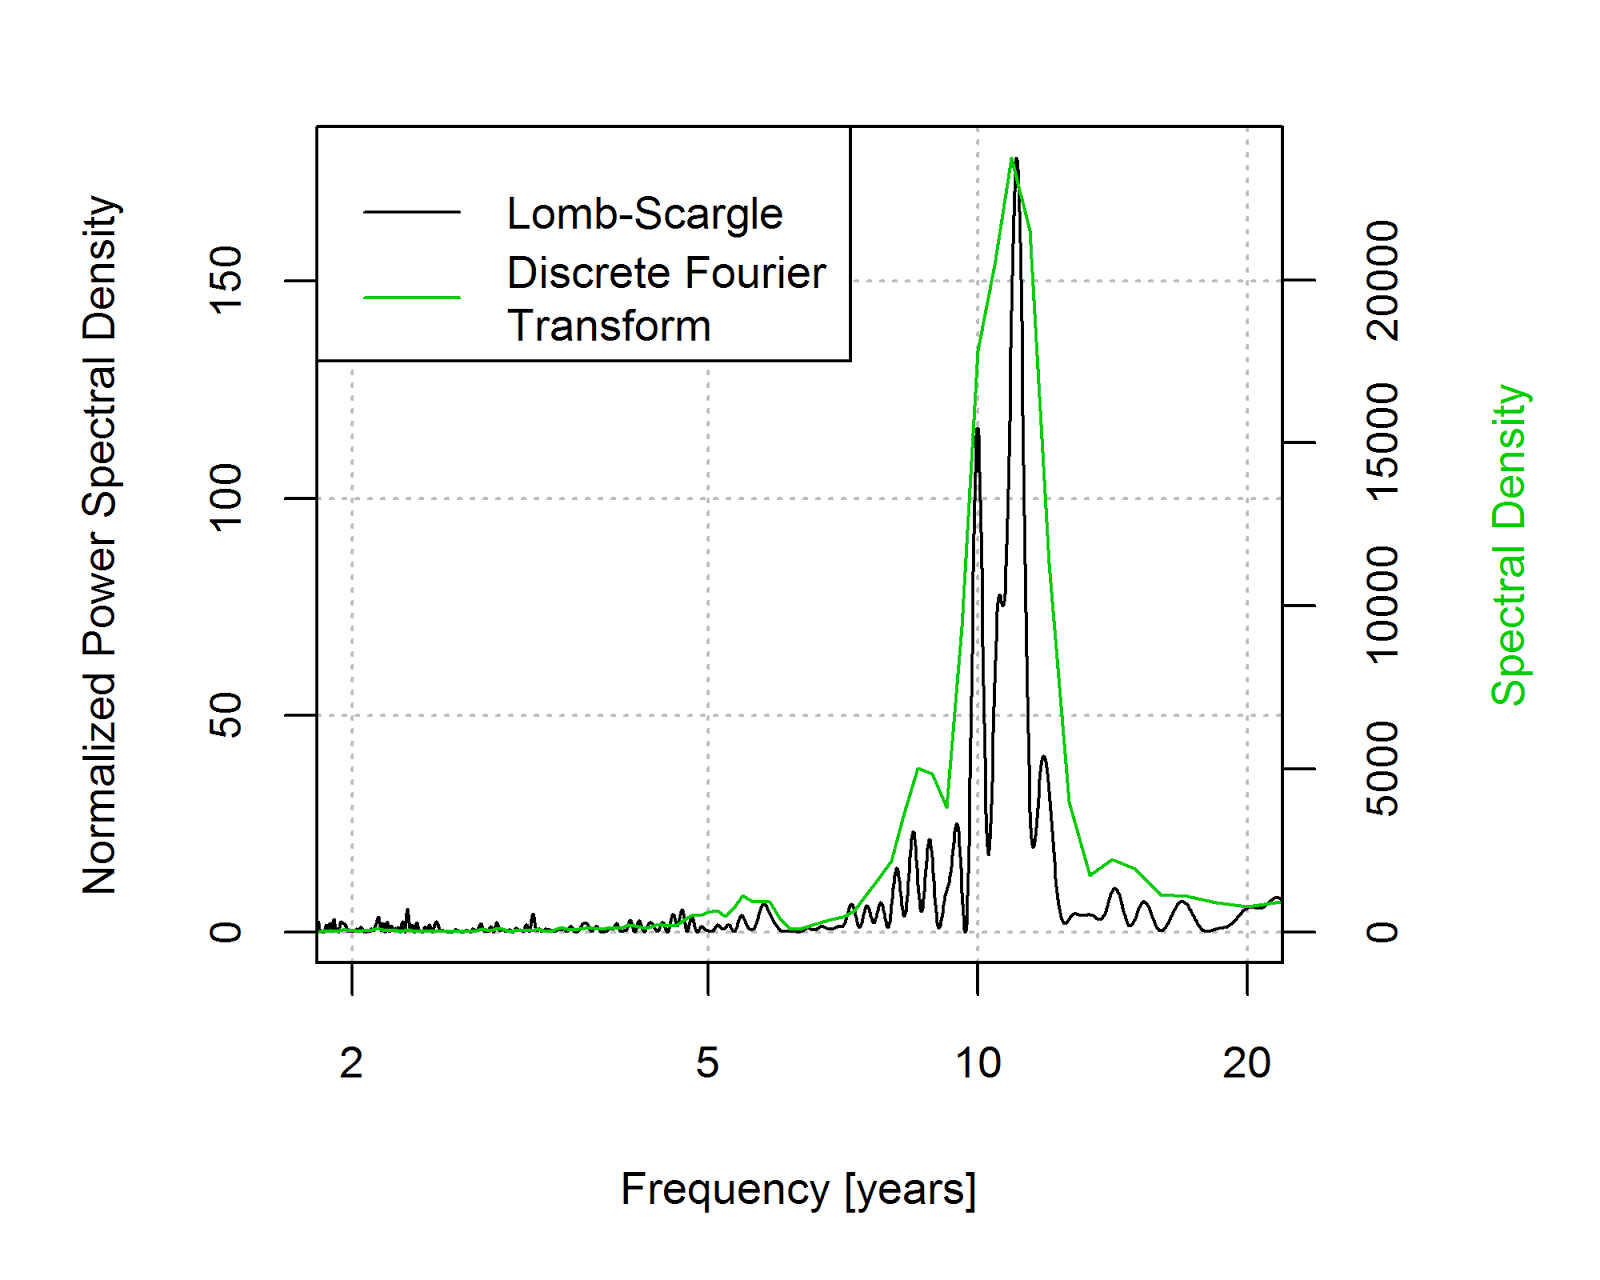
\includegraphics[width = 0.6\textwidth]{lomb_vs_FFT.png}
    \caption{The Lomb–Scargle Periodogram works better with variable intervals.}
  \end{figure}
\end{frame}

\begin{frame}{Train frequency over increasing input step}
\begin{figure}
    \centering
    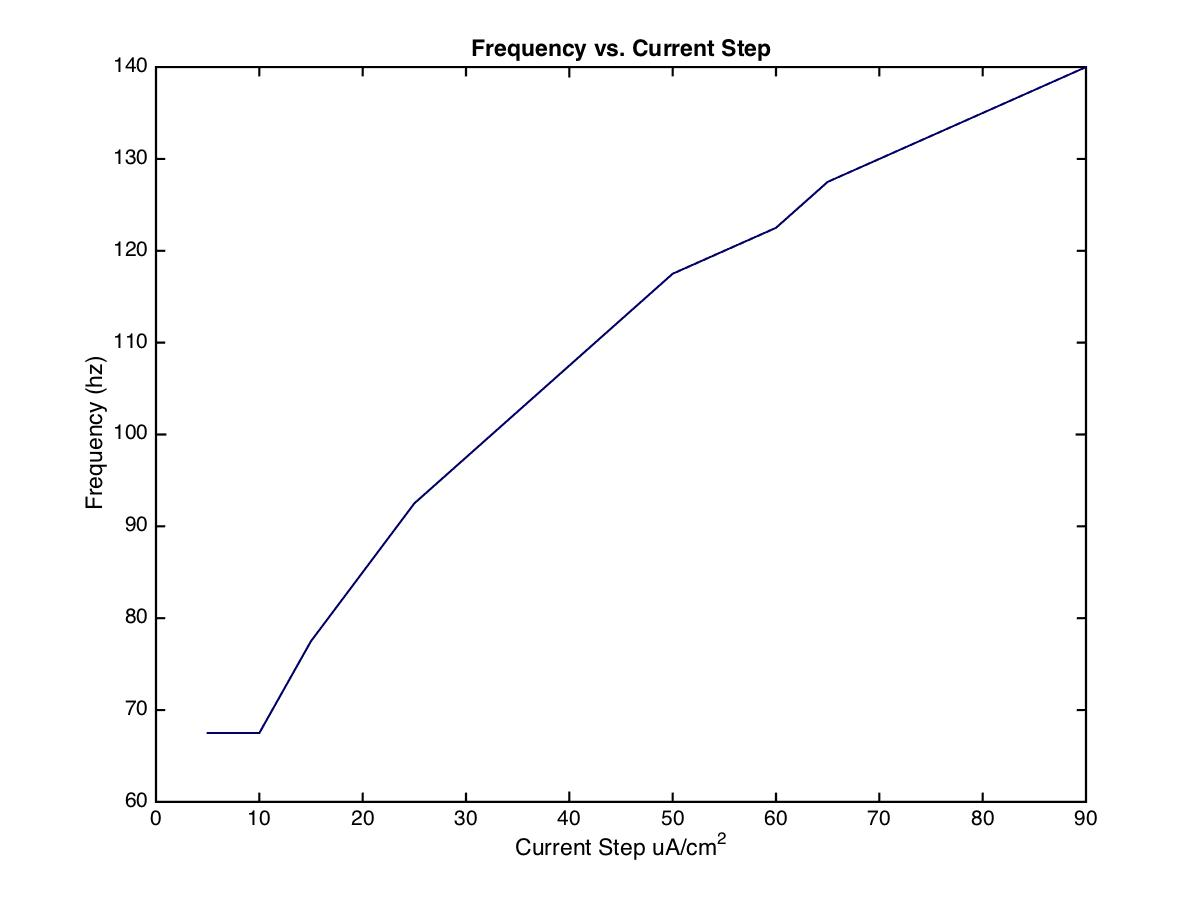
\includegraphics[width = 0.8\textwidth]{./images/freqvscurrent.jpg}
    \caption{Graph of train frequency over increasing input step}
  \end{figure}

\end{frame}


% Experimental design
\begin{frame}{Issues with precision approximation}
  % Precision required
  % Simulation very sensitive to minute perturbations
  % Base precision settings appear to be calibrated for fast approximations of
  % single action potentials at lower currents
  % Needed much higher precision to get reasonable values
  % Diagnosis used stepping by 0.1 increments at very high current
  \begin{figure}
    \centering
    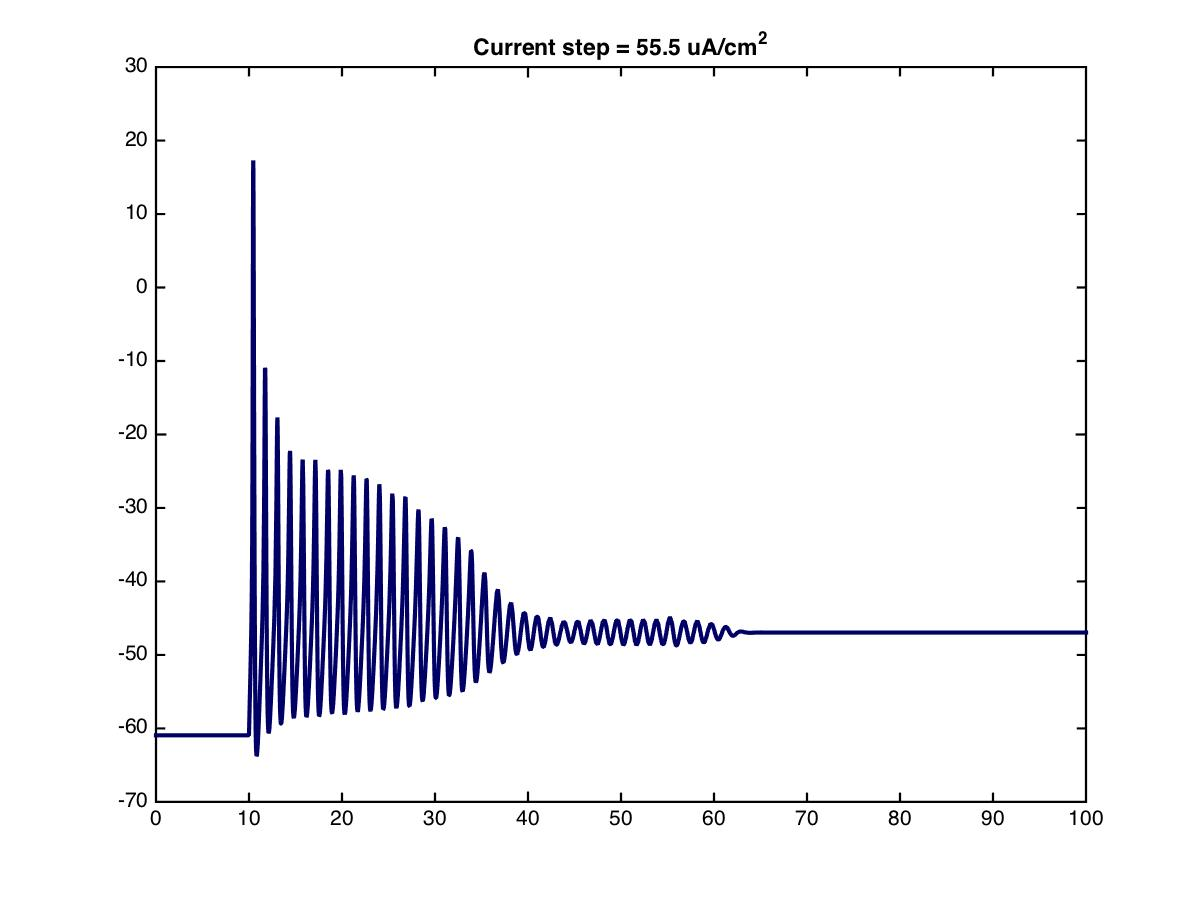
\includegraphics[width = 0.4\textwidth]{./images/current55p5.jpg}
    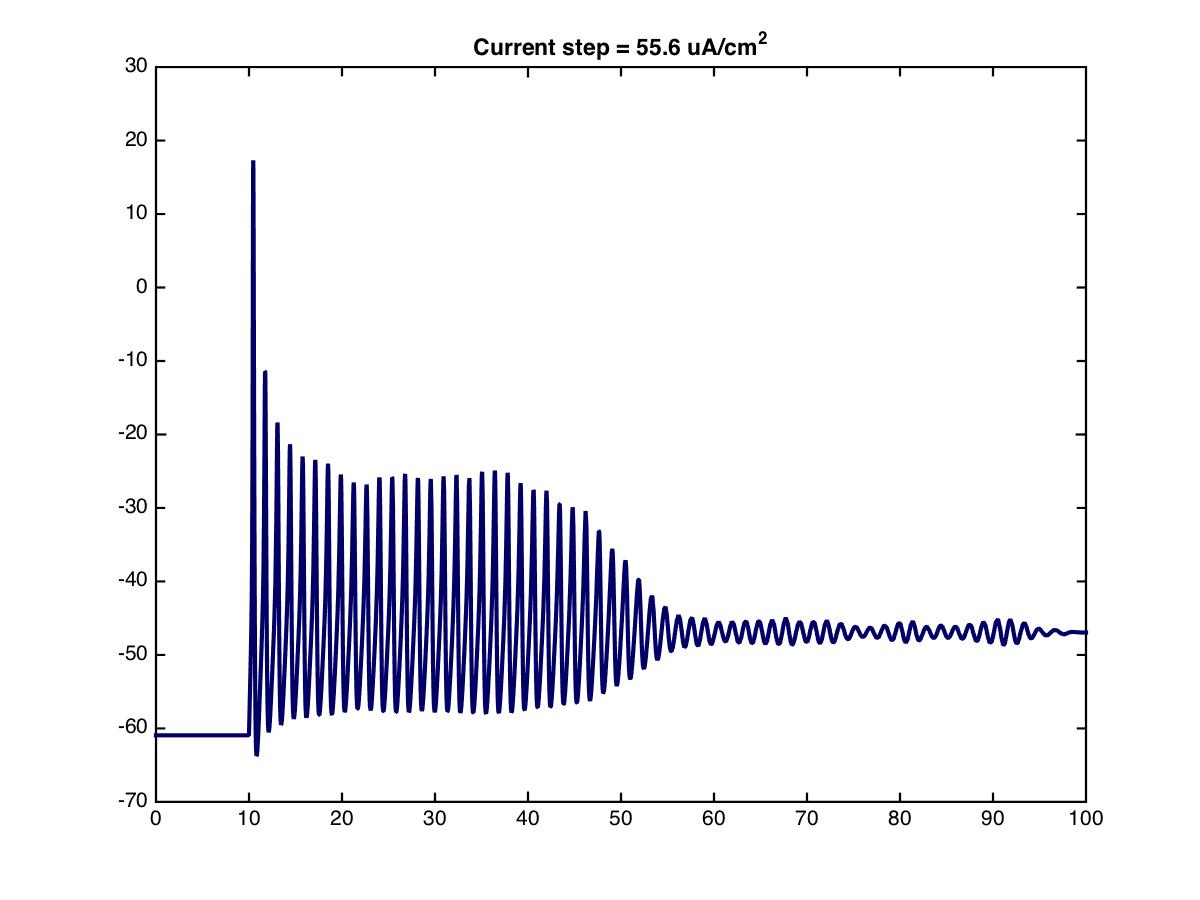
\includegraphics[width = 0.4\textwidth]{./images/current55p6.jpg}
    \caption{Incorrect behavior due to low precision}
  \end{figure}
\end{frame}

\begin{frame}{References}
\begin{enumerate}
\item Weiss, T. F. (1995).Cellular Biophysics. Volume 1: Transport, MIT Press.
\item Weiss, T. F. (1995).Cellular Biophysics. Volume 2: Electrical Properties, MIT Press.
\item Blaustein, M.P., Kao, J.P.Y., Matteson, D.R. (2012). Cellular Physiology and Neurophysiology, 2nd edition, Elsevier-Mosby. 
\item Gerstner, Wulfram, and Werner M. Kistler. Spiking neuron models: Single neurons, populations, plasticity. Cambridge university press, 2002.
\item Press, William H., and George B. Rybicki. "Fast algorithm for spectral analysis of unevenly sampled data." The Astrophysical Journal 338 (1989): 277-280.
\end{enumerate}
\end{frame}
\end{document}
